\documentclass[hidelinks,12pt]{article}
\usepackage[left=0.25cm,top=1cm,right=0.25cm,bottom=1cm]{geometry}
%\usepackage[landscape]{geometry}
\textwidth = 20cm
\hoffset = -1cm
\usepackage[utf8]{inputenc}
\usepackage[spanish,es-tabla]{babel}
\usepackage[autostyle,spanish=mexican]{csquotes}
\usepackage[tbtags]{amsmath}
\usepackage{nccmath}
\usepackage{amsthm}
\usepackage{amssymb}
\usepackage{mathrsfs}
\usepackage{graphicx}
\usepackage{subfig}
\usepackage{standalone}
\usepackage[outdir=./Imagenes/]{epstopdf}
\usepackage{siunitx}
\usepackage{physics}
\usepackage{color}
\usepackage{float}
\usepackage{hyperref}
\usepackage{multicol}
%\usepackage{milista}
\usepackage{anyfontsize}
\usepackage{anysize}
%\usepackage{enumerate}
\usepackage[shortlabels]{enumitem}
\usepackage{capt-of}
\usepackage{bm}
\usepackage{relsize}
\usepackage{placeins}
\usepackage{empheq}
\usepackage{cancel}
\usepackage{wrapfig}
\usepackage[flushleft]{threeparttable}
\usepackage{makecell}
\usepackage{fancyhdr}
\usepackage{tikz}
\usepackage{bigints}
\usepackage{scalerel}
\usepackage{pgfplots}
\usepackage{pdflscape}
\pgfplotsset{compat=1.16}
\spanishdecimal{.}
\renewcommand{\baselinestretch}{1.5} 
\renewcommand\labelenumii{\theenumi.{\arabic{enumii}})}
\newcommand{\ptilde}[1]{\ensuremath{{#1}^{\prime}}}
\newcommand{\stilde}[1]{\ensuremath{{#1}^{\prime \prime}}}
\newcommand{\ttilde}[1]{\ensuremath{{#1}^{\prime \prime \prime}}}
\newcommand{\ntilde}[2]{\ensuremath{{#1}^{(#2)}}}

\newtheorem{defi}{{\it Definición}}[section]
\newtheorem{teo}{{\it Teorema}}[section]
\newtheorem{ejemplo}{{\it Ejemplo}}[section]
\newtheorem{propiedad}{{\it Propiedad}}[section]
\newtheorem{lema}{{\it Lema}}[section]
\newtheorem{cor}{Corolario}
\newtheorem{ejer}{Ejercicio}[section]

\newlist{milista}{enumerate}{2}
\setlist[milista,1]{label=\arabic*)}
\setlist[milista,2]{label=\arabic{milistai}.\arabic*)}
\newlength{\depthofsumsign}
\setlength{\depthofsumsign}{\depthof{$\sum$}}
\newcommand{\nsum}[1][1.4]{% only for \displaystyle
    \mathop{%
        \raisebox
            {-#1\depthofsumsign+1\depthofsumsign}
            {\scalebox
                {#1}
                {$\displaystyle\sum$}%
            }
    }
}
\def\scaleint#1{\vcenter{\hbox{\scaleto[3ex]{\displaystyle\int}{#1}}}}
\def\bs{\mkern-12mu}



\title{Expansión del potencial de Coulomb \\ {\large Tema 4}\vspace{-3ex}}
\author{M. en C. Gustavo Contreras Mayén}
\date{ }

\pagestyle{fancy}
\fancyhf{}
\rhead{Curso MAF}
\lhead{\leftmark}
\rfoot{\thepage}
\setlength{\headheight}{16pt}%

\def\changemargin#1#2{\list{}{\rightmargin#2\leftmargin#1}\item[]}
\let\endchangemargin=\endlist 


\begin{document}
\maketitle
\fontsize{14}{14}\selectfont
\tableofcontents
\newpage

\section{Introducción.}

Del curso de electromagnetismo se conoce que el cálculo del potencial eléctrico es un problema simple, pues se conoce una forma analítica para su cálculo, sin embargo, si en el sistema de interés no se tienen las simetrías geométricas para resolver la ecuación integral, el problema se complica seriamente.
\par
En este material, se presenta una alternativa para su cálculo haciendo uso del teorema de adición de los armónicos esféricos y por consiguiente de los polinomios asociados de Legendre.

\section{Potencial de Couloumb.}

El potencial eléctrico queda determinado por:
\begin{align}
\Phi (\va{r}) = \scaleint{6ex} \dfrac{\rho(\va{r})}{\abs{\va{r}^{\, \prime} - \va{r}}} \dd{V^{\prime}}
\label{eq:ecuacion_01}
\end{align}
Las coordenadas $\va{r}^{\, \prime}$ indican las coordenadas del punto fuente, es decir, la coordenadas donde la distribución de carga está definida, y las coordenadas $\va{r}$ son las coordenadas de campo, es decir, todas las posibles posiciones donde se realizará una medición del potencial eléctrico (ver la figura 1).
\begin{figure}[H]
    \centering
    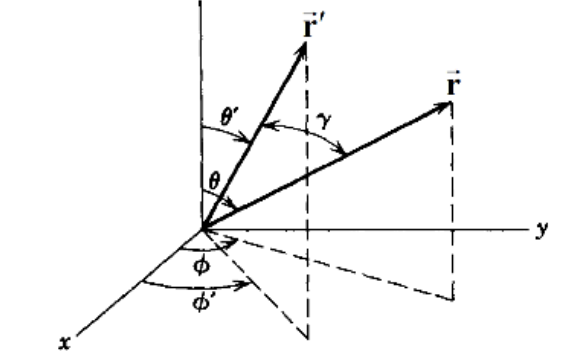
\includegraphics[scale=0.5]{Imagenes/Potencial_Coulomb.png}
    \caption{Sistema de coordenadas empleado en la expansión del potencial de Coulomb.}
    \label{fig:figura_01}
\end{figure}

Trabajaremos la ec. (\ref{eq:ecuacion_01}) con la finalidad de facilitar la integración:
\begin{align}
\begin{aligned}
\Phi (\va{r}) &= \scaleint{6ex} \dfrac{\rho(\va{r})}{\abs{\va{r}^{\, \prime} - \va{r}}} \dd{V^{\prime}} = \\[0.5em]
&= \scaleint{6ex} \dfrac{\rho(\va{r})}{\sqrt{r^{\, \prime 2} + r - 2 r^{\prime} \cdot r}} \dd{V^{\prime}} = \\[0.5em]
&= \scaleint{6ex} \dfrac{\rho(\va{r})}{\sqrt{r^{\, \prime 2} + r - 2 r^{\prime} \, r \, \cos \gamma }} \dd{V^{\prime}}
\end{aligned}
\label{eq:ecuacion_02}
\end{align}
Indicando con:
\begin{align*}
r_{<} = \min \left\{ r, r^{\prime} \right\} \hspace{1.5cm} r_{>} = \max \left\{ r, r^{\prime} \right\}
\end{align*}
expandimos el denominador de la ec. (\ref{eq:ecuacion_02}):
\begin{align}
\Phi (\va{r}) &= \dfrac{1}{r_{>}} \, \scaleint{10ex} \dfrac{\rho (\va{r}^{\, \prime})}{\sqrt{1 + \bigg( \dfrac{r_{<}}{r_{>}} \bigg)^{2} - 2 \dfrac{r_{<}}{r_{>}} \, \cos \gamma}} \dd{V^{\prime}} = \\[0.5em]
&= \scaleint{6ex} \rho(\va{r}) \, \dfrac{1}{\sqrt{r^{\, \prime 2} + r - 2 r^{\prime} \, r \, \cos \gamma }} \dd{V^{\prime}}
\label{eq:ecuacion_03}
\end{align}
donde:
\begin{align*}
\cos \gamma = \va{r} \cdot \va{r}^{\, \prime} = \cos \theta \cos \theta^{\prime} +  \sin \theta \sin \theta^{\prime} \cos (\varphi - \varphi^{\prime})
\end{align*}
Notemos que el denominador de la eq. (\ref{eq:ecuacion_03}) es \emph{la función generadora de los polinomios ordinarios de Legendre}, por lo cual, podemos reescribir el potencial como:
\begin{align}
\Phi (\va{r}) &= \dfrac{1}{r_{>}} \, \scaleint{10ex} \dfrac{\rho (\va{r}^{\, \prime})}{\sqrt{1 + \bigg( \dfrac{r_{<}}{r_{>}} \bigg)^{2} - 2 \dfrac{r_{<}}{r_{>}} \, \cos \gamma}} \dd{V^{\prime}} = \\[0.5em]
&= \dfrac{1}{r_{>}} \nsum_{l=0}^{\infty} \scaleint{8ex} \bigg( \dfrac{r_{<}}{r_{>}} \bigg)^{l} \, \rho (\va{r}^{\, \prime}) \, P_{l} (\cos \gamma) \dd{V}^{\prime}
\label{eq:ecuacion_04}
\end{align}
Para realizar la integración de la ec. (\ref{eq:ecuacion_04}) reescribimos el $\cos \gamma$, en términos de las variables $\va{r}$ y $\va{r}^{\, \prime}$, para ello usamos el teorema de adición de los armónicos esféricos:
\begin{align}
P_{l} (\cos \gamma) = \dfrac{4 \pi}{2 \, l + 1} \nsum_{m=-l}^{l} Y_{l}^{m} (\theta^{\prime}, \varphi^{\prime})^{*} \, Y_{l}^{m} (\theta, \varphi)
\label{eq:ecuacion_05}    
\end{align}
entonces al sustituir la ec. (\ref{eq:ecuacion_04}) en la ec. (\ref{eq:ecuacion_05}), obtenemos:
\begin{align}
\Phi (\va{r}) =  \nsum_{l=0}^{\infty} \, \nsum_{m=-l}^{l} \dfrac{4 \pi}{2 l {+} 1} \, Y_{l}^{m} (\theta, \varphi) \, \scaleint{8ex} \dfrac{(r_{<})^{l}}{r_{>}^{l+1}} \, \rho (\va{r}^{\, \prime}) \, Y_{l}^{m} (\theta^{\prime}, \varphi^{\prime})^{*} \, r^{\prime 2} \sin \theta^{\prime} \dd{r}^{\prime} \dd{\theta}^{\prime} \dd{\varphi}^{\prime}
\label{eq:ecuacion_06}
\end{align}
La integración de la ec. (\ref{eq:ecuacion_06} se realiza por casos, tomando en cada uno la correspondiente variable primada en $r_{<}$ y $r_{>}$, aunque la ec.(\ref{eq:ecuacion_06}) es válida para cualquier distribución de carga, sin embargo estos desarrollos tienen su mayor beneficio en sistemas donde el punto fuente está lejos del punto campo, en este caso la estructura de la configuración de carga es irrelevante y se aprecia como un sistema de cargas puntuales. Este proceso se conoce en la literatura como \emph{desarrollo multipolar} y es la base del estudio de materiales dieléctricos y una de sus aplicaciones es la construcción de la zona de radiación.

\section{Desarrollo multipolar.}

Este caso particular corresponde a $\abs{\va{r}^{\, \prime}} = r_{<}$, de tal manera que la ec. (\ref{eq:ecuacion_06}) se reescribe como:
\begin{align}
\begin{aligned}
\Phi (\va{r}) &=  \nsum_{l=0}^{\infty} \nsum_{m=-l}^{l} \dfrac{4 \pi}{2 l {+} 1} \dfrac{Y_{l}^{m} (\theta, \varphi)}{r^{l+1}} \scaleint{8ex} \rho (\va{r}^{\, \prime}) r^{l+2} Y_{l}^{m} (\theta^{\prime}, \varphi^{\prime})^{*} \sin \theta^{\prime} \dd{r}^{\prime} \dd{\theta}^{\prime} \dd{\varphi}^{\prime} = \\[0.5em]
&= \nsum_{l=0}^{\infty} \nsum_{m=-l}^{l} \dfrac{4 \pi}{2 l {+} 1} \dfrac{Y_{l}^{m} (\theta, \varphi)}{r^{l+1}} \bigg[ \scaleint{6ex} \rho (\va{r}^{\, \prime}) r^{l+2} Y_{l}^{m} (\theta^{\prime}, \varphi^{\prime})^{*} \sin \theta^{\prime} \dd{r}^{\prime} \dd{\theta}^{\prime} \dd{\varphi}^{\prime} \bigg] = \\[0.5em]
&= \nsum_{l=0}^{\infty} \nsum_{m=-l}^{l} \dfrac{4 \pi}{2 l {+} 1} \, \dfrac{q_{l, m} \, Y_{l}^{m}(\theta, \varphi)}{r^{l+1}}
\end{aligned}
\label{eq:ecuacion_07}
\end{align}
siendo $q_{l,m}$ los momentos multipolares y están definidos por el término entre corchetes.
\par
Para ilustrar la ec. (\ref{eq:ecuacion_07}), resolvamos un caso particular para la siguiente distribución de carga:
\begin{figure}[H]
    \centering
    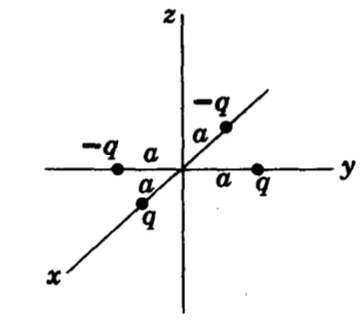
\includegraphics[scale=0.6]{Imagenes/Desarrollo_multipolar_4_cargas.png}
    \caption{Distribución de cargas para el ejercicio.}
    \label{fig:figura_02}
\end{figure}

Calculamos el potencial eléctrico de la distribución de carga de la figura (\ref{fig:figura_02}), para este propósito seguimos la Ec.(\ref{eq:ecuacion_07}), el primer requisito para el cálculo, es conocer la densidad de carga, recordando que la distribución de carga de una carga puntual es $\rho (\va{r}) = q \, \delta (\va{r})$, en el caso de la figura (\ref{fig:figura_02}) se tiene que:
\begin{align}
\rho(\va{r}) &= q \, \big[ \delta (x - a) \delta(y) \delta(z) -  \delta (x + a) \delta(y) \delta(z) + \\[0.5em]
&+ \delta (x) \delta(y - a) \delta(z) - \delta (x) \delta(y + a) \delta(z) \big]
\label{eq:ecuacion_08}
\end{align}
Usando la transformación de la delta de Dirac a coordenadas esféricas, la ec. (\ref{eq:ecuacion_08}) la escribimos como:
\begin{align}
\begin{aligned}[b]
\rho(\va{r}) &= \dfrac{q}{r^{2}} \times \bigg[ \delta(r {-} a) \delta(\cos \theta) \delta(\varphi) {-} \delta(r {-} a) \delta(\cos \theta) \delta(\varphi {-} \pi) + \\[0.5em]
&+ \delta(r {-} a) \delta(\cos \theta) \delta \bigg(\varphi {-} \dfrac{\pi}{2} \bigg) {-} \delta(r {-} a) \delta(\cos \theta) \delta \bigg( \varphi {-} \dfrac{3 \pi}{2} \bigg) \bigg] = \\[0.5em]
&= \dfrac{q}{r^{2}} \delta(r {-} a) \delta(\cos \theta) \bigg[ \delta \big(\varphi \big) {-} \delta \big(\varphi {-} \pi \big) {+} \delta \bigg( \varphi {-} \dfrac{\pi}{2} \bigg) {-} \delta \bigg(\varphi {-} \dfrac{3 \pi}{2} \bigg) \bigg]
\end{aligned}
\label{eq:ecuacion_09}
\end{align}
Sustituyendo la ec. (\ref{eq:ecuacion_09}) en la ec. (\ref{eq:ecuacion_07}), obtenemos el cálculo de los momentos multipolares:
\begin{align}
\begin{aligned}[b]
q_{l,m} &= \scaleint{5ex} \rho (\va{r}) \, r^{l+2} \, Y_{l}^{m} (\theta, \varphi)^{*} \, \sin \theta \dd{r} \dd{\theta} \dd{\varphi} = \\[0.5em]
&= \scaleint{5ex}_{\bs 0}^{2 \pi} \scaleint{5ex}_{\bs 0}^{\pi} \scaleint{5ex}_{\bs 0}^{\infty} q \, \delta(r {-} a) \delta(\cos \theta) \times \\[0.5em]
&\times \bigg[ \delta \big(\varphi \big) {-} \delta \big(\varphi {-} \pi \big) {+} \delta \bigg( \varphi {-} \dfrac{\pi}{2} \bigg) {-} \delta \bigg(\varphi {-} \dfrac{3 \pi}{2} \bigg) \bigg] \times \\[0.5em]
&\times r^{l} \, Y_{l}^{m} (\theta, \varphi)^{*} \sin \theta \dd{r} \dd{\theta} \dd{\varphi} = \\[0.5em]
&= q \, a^{l} \scaleint{5ex}_{\bs 0}^{2 \pi} \scaleint{5ex}_{\bs 0}^{\pi} \delta(\cos \theta) \bigg[ \delta \big(\varphi \big) {-} \delta \big(\varphi {-} \pi \big) {+} \delta \bigg( \varphi {-} \dfrac{\pi}{2} \bigg) {-} \delta \bigg(\varphi {-} \dfrac{3 \pi}{2} \bigg) \bigg] \times \\[0.5em]
&\times \, \textcolor{blue}{Y_{l}^{m} (\theta, \varphi)^{*}} \sin \theta \dd{\theta} \dd{\varphi}
\end{aligned}
\label{eq:ecuacion_10}
\end{align}
Para realizar la integración de la ec. (\ref{eq:ecuacion_10}), debemos de escribir la forma explícita del armónico esférico $\textcolor{blue}{Y_{l}^{m} (\theta, \varphi)^{*}}$:
\begin{align}
\begin{aligned}[b]
\textcolor{blue}{Y_{l}^{m} (\theta, \varphi)^{*}} &= (-1)^{m} \, Y_{l}^{-m} (\theta, \varphi) = \\[0.5em]
&= (-1)^{m} \, \sqrt{\dfrac{2 l + 1}{4 \pi} \, \dfrac{(l + m)!}{(l - m)!}} \, \textcolor{red}{P_{l}^{-m} (cos \theta)} \, e^{-i m \varphi} = \\[0.5em]
&= (-1)^{m} \, \sqrt{\dfrac{2 l + 1}{4 \pi} \, \dfrac{(l + m)!}{(l - m)!}} \textcolor{red}{\bigg[ (-1)^{m} \dfrac{(l - m)!}{(l + m)!} P_{l}^{m} (\cos \theta) \bigg]} \, e^{-i m \varphi} = \\[0.5em]
&= \sqrt{\dfrac{2 l + 1}{4 \pi} \, \dfrac{(l - m)!}{(l + m)!}} \, P_{l}^{m} (\cos \theta) \, e^{-i m \varphi} 
\end{aligned}
\label{eq:ecuacion_11}
\end{align}
Sustituyendo la ec. (\ref{eq:ecuacion_11}) en la ec. (\ref{eq:ecuacion_10}), tendremos que:
\begin{align*}
q_{l, m} &= q \, a^{l} \scaleint{5ex}_{\bs 0}^{2 \pi} \scaleint{5ex}_{\bs 0}^{\pi} \delta(\cos \theta) \bigg[ \delta \big(\varphi \big) {-} \delta \big(\varphi {-} \pi \big) {+} \delta \bigg( \varphi {-} \dfrac{\pi}{2} \bigg) {-} \delta \bigg(\varphi {-} \dfrac{3 \pi}{2} \bigg) \bigg] \times \\[0.5em]
&\times \, \textcolor{blue}{Y_{l}^{m} (\theta, \varphi)^{*}} \sin \theta \dd{\theta} \dd{\varphi} = \\[0.5em]
&= q \, a^{l} \scaleint{5ex}_{\bs 0}^{2 \pi} \scaleint{5ex}_{\bs 0}^{\pi} \delta(\cos \theta) \bigg[ \delta \big(\varphi \big) {-} \delta \big(\varphi {-} \pi \big) {+} \delta \bigg( \varphi {-} \dfrac{\pi}{2} \bigg) {-} \delta \bigg(\varphi {-} \dfrac{3 \pi}{2} \bigg) \bigg] \times \\[0.5em]
&\times \, \textcolor{red}{\sqrt{\dfrac{2 l + 1}{4 \pi} \, \dfrac{(l - m)!}{(l + m)!}} \, P_{l}^{m} (\cos \theta) \, e^{-i m \varphi}} \sin \theta \dd{\theta} \dd{\varphi} = \\[0.5em]
&= q \, a^{l} \sqrt{\dfrac{2 l + 1}{4 \pi} \, \dfrac{(l - m)!}{(l + m)!}} \, P_{l}^{m} (0) \times \\[0.5em]
&\times \scaleint{6ex} \bigg[ \delta \big(\varphi \big) {-} \delta \big(\varphi {-} \pi \big) {+} \delta \bigg( \varphi {-} \dfrac{\pi}{2} \bigg) {-} \delta \bigg(\varphi {-} \dfrac{3 \pi}{2} \bigg) \bigg] \, e^{-i m \varphi} \dd{\varphi} = \\[0.5em]
&= q \, a^{l} \sqrt{\dfrac{2 l + 1}{4 \pi} \, \dfrac{(l - m)!}{(l + m)!}} \, P_{l}^{m} (0) \bigg[ 1 - e^{- i \pi m } + e^{- i  \dfrac{\pi}{2} m} - e^{- i  \dfrac{3 \pi}{2} m} \bigg] = \\[0.5em]
&= q \, a^{l} \sqrt{\dfrac{2 l + 1}{4 \pi} \, \dfrac{(l - m)!}{(l + m)!}} \, P_{l}^{m} (0) \big[ 1 - (-1)^{m} \big] \, \big[ 1 - i^{m} \big]
\end{align*}
Por lo que el potencial se reescribe como:
\begin{align}
\begin{aligned}
\Phi(\va{r}) &= \nsum_{l=0}^{\infty} \nsum_{m=-l}^{l} \dfrac{4 \pi}{2 l {+} 1} \times \\[0.5em]
&\times \bigg[ q \, a^{l} \sqrt{\dfrac{2 l + 1}{4 \pi} \, \dfrac{(l - m)!}{(l + m)!}} \, P_{l}^{m} (0) \big[ 1 - (-1)^{m} \big] \, \big[ 1 - i^{m} \big] \bigg] \, \dfrac{Y_{l}^{m}(\theta, \varphi)}{r^{l+1}}
\end{aligned}
\label{eq:ecuacion_12}
\end{align}
Que es lo que se pedía en el ejercicio, observa que para un observador en el eje $z$, \emph{el potencial es nulo},  que es lo que convencionalmente se muestra en los libros elementales de electromagnetismo .
\end{document}